\documentclass[%
 sor,
 jor,
 amsmath,amssymb,
 reprint,
]{revtex4-2}
\usepackage{ulem}
\usepackage{graphicx}
\usepackage{xcolor}
\usepackage{siunitx}
\usepackage{dcolumn}
\usepackage{bm}
\usepackage{amsmath, amssymb, amsfonts}
\usepackage{placeins}
\usepackage{float}
\usepackage{pgfplots}
\pgfplotsset{compat=1.17}

\graphicspath{{./photos/}}

\begin{document}

\title{Experiment 2\\Thermal Expansion of Metals}

\author{Aumshree P. Shah\\20231059}
\altaffiliation{\color{red}aumshree.pinkalbenshah@students.iiserpune.ac.in}
\date{\today}

\begin{abstract}
\centering
In this experiment, we try to determine the thermal expansion coefficient of different metals.
\end{abstract}

\maketitle

\section{Theory and Procedure}
\subsection{Apparatus}
\small
\begin{minipage}{0.48\textwidth}
\begin{itemize}
	\item[] Thermal Expansion Apparatus
	\item[] Brass, Aluminium, Copper and Steel rods 
\end{itemize}
\end{minipage}
\begin{minipage}{0.48\textwidth}
\begin{itemize}
	\item[] Steam generator and electric heater
		\item[] Thermometer for temperature measurements
\end{itemize}
\end{minipage}
\subsection{Theory}
When a solid is heated, its length increases. This expansion is approximately linear for small temperature ranges:
\begin{equation}
L = L_0 (1 + \alpha \Delta T)
\end{equation}
where $L$ is the final length, $L_0$ the initial length, $\alpha$ the coefficient of thermal expansion, and $\Delta T$ the temperature change.
The above formula can simply be written as: $$\Delta L = L \alpha \Delta T $$ For this experiment we use thermal expansion apparatus as shown in the image:\\

\begin{center}
\includegraphics[width=0.9\textwidth, trim={0 31cm 0 0},clip]{apparatus}
\end{center}

\subsection{Procedure}
\begin{enumerate}
	\item Place the rod in the apparatus.
	\item Fix all the screws in proper position to make the road stable. 
	\item Measure the temperature of the rod along the ends and the center for better accuracy.
	\item Now fix the steam tubes in their proper position.
	\item When everything is measured, measure the length of the road between the two clamps.
	\item Start the induction and when the steam passes through the rod, measure the expansion of the rod using the spherometer. 
	\item Let the apparatus cool before putting in another rod and repeat this for different materials and different rods.
\end{enumerate}
\subsubsection{Precautions}
\begin{itemize}
	\item Ensure to use thermal gloves, this helps reduce the heat flow from our hand to apparatus
	\item After measuring the expansion, sprinkle water or give enough time for the apparatus to cool (we used wet paper towels to cool the apparatus)
	\item Ensure the screws are tight enough. 
	\item Measure the length of the rod after fixing the screws, measuring the length before may change its value when fixing the screws.
	\item Use different rods, when using the same material to reduce any instrumental error from material.
\end{itemize}
\subsubsection{Calibration}
We start by calibrating the apparatus to see weather the apparatus is working or not. For this we shall use copper rods whose thermal expansion coefficient is known; $\alpha_{\text{copper}} = 16.6 \times 10^{-6} \si{\per\celsius}$\footnote{Reference: \cite{alpha}}. We place the rods in the apparatus and measure its length ($L$), change in length ($\Delta L$) and temperature across the rod, which may not be the same so we take multiple values to reduce error. 
\begin{center}
\begin{tabular}{ |c|c|c|c| } 
 \hline
	Material 	& $T_i (\si{\celsius})$ 	& $L (\si{\centi\meter})$) 	& $\Delta L (10^{-5}\si{\meter})$ \\ 
	\hline
	Copper		& 24.0 				& 59.0 				& 75\\
	Copper		& 25.5-24.5-25.5 		& 59.7				& 74\\	
 \hline
\end{tabular}
\end{center}
Now using the known $\alpha_{\text{copper}}$ we calculate the temperature of rods in equilibrium as: 
\begin{center}
\begin{tabular}{ |c|c|c|c|c|c| } 
 \hline
 Material 	& $T_i (\si{\celsius})$ 	& $L (\si{\centi\meter})$) 	& $\Delta L (10^{-5}\si{\meter})$ & $\alpha (10^{-6}\si{\per\celsius})$	& $T_f (\si{\celsius})$ \\ 
	\hline
 Copper		& 24.0 				& 59.0 				& 75 	& 16.6 & 99.6\\
 Copper		& 25.5-24.5-25.5 		& 59.7				& 74 	& 16.6 & 99.3\\	
 \hline
\end{tabular}
\end{center}
From this data and Appendix-B and we conclude that the temperature of rods in equilibrium is $= 99\pm1~\si{\celsius}$; which we shall take as the final temperature to calculate coefficient of thermal expansion of the other materials. 


\section{Observations}

\begin{table}[h]
\centering
\begin{tabular}{|c|ccc|}
    \hline
    Material & $T_i$ (\si{\celsius})  & Length (cm) & $\Delta L$ ($10^{-5}$ m)\\
    \hline
    Copper 	& 24.0     & 59.8 & 75 \\
    Copper 	& 25.5-24.5-25.5 & 59.7 & 74\\
    Aluminium 	& 24.0-23.0-24.7 & 59.9 & 105\\
    Brass 	& 24.1-23.2-24.3 & 59.7 & 85 \\
    Steel 	& 22.1-24.8-20.5 & - & 74 \\
    Aluminium 	& 24.3-23.7-24.3 & 59.8 & 104\\
    Brass 	& 23.7-22.4-24.3 & 60.0 & 85 \\
    Steel 	& 24.6-25.3 & 59.9 & 76 \\
    Brass	& 24.8-25.3 & 60.1 & 86 \\
    Steel 	& 23.3-23.5 & 59.7 & 76 \\ 
    \hline
\end{tabular}
\caption{Data taken on 11 Mar 2025, the variables represents the property as described in the theory. The '-' value is assumed to be 60.0 cm.}

\end{table}
\noindent Least count of scale: \uline{0.1 cm}  \\
Least count of thermometer:\uline{ 0.1 $\si{\celsius}$ }\\
Least count of spherometer:\uline{$10^{-5}$ m } \\


\section{Uncertainties and Error Sources}
\subsection{Measurement Uncertainties}
\begin{itemize}
    \item \textbf{Length Measurements:} Estimated uncertainty of $\pm 0.1$ cm due to not proper method of viewing, expansion uncertainty of $\pm 5\times 10^{-6}$ m.
    \item \textbf{Temperature Measurements:} Uncertainty of $\pm 0.05$ \si{\kelvin} due to instrument resolution.
\end{itemize}



\section{Calculation and Error Analysis}
\subsection{Error Propagation}
From the length and temperature uncertainty, and using Equation-1 uncertainty in $\alpha$, by the basic formula for error propagation$^{[1]}$ will propogate as .:
\[
\sigma_{\alpha} = \alpha \sqrt{\left( \frac{\sigma_{\Delta L}}{\Delta L} \right)^2 + \left( \frac{\sigma_L}{L} \right)^2 + \left( \frac{\sigma_{\Delta T}}{\Delta T} \right)^2}
\]
where $\sigma_{\Delta L}, \sigma_L, \sigma_{\Delta T}$ are the uncertainties in expansion length, initial length, and temperature difference, respectively.

\subsection{Calculation}
We calculate the value of $\alpha$ of all data points and their uncertainity from hte above formul,  we get (Refer to [3] for calculations):

\begin{table}[h]
\centering
\begin{tabular}{ccc}
\hline
Material & $\alpha$ (\si{1/\degreeCelsius}) \\
\hline
Aluminium & $(2.33 \pm 0.02) \times 10^{-5}$ \\
Aluminium & $(2.32\pm 0.02) \times 10^{-5}$ \\
Brass & $(1.90\pm 0.02) \times 10^{-5}$ \\
Brass & $(1.88\pm 0.02) \times 10^{-5}$ \\
Brass & $(1.92\pm 0.02 \times 10^{-5}$ \\
Copper & $(1.67\pm 0.02) \times 10^{-5}$ \\
Copper & $(1.68\pm 0.02) \times 10^{-5}$ \\
Steel & $(1.61\pm 0.02) \times 10^{-5}$ \\
Steel & $(1.71\pm 0.02) \times 10^{-5}$ \\
Steel & $(1.68\pm 0.02) \times 10^{-5}$ \\

\hline


\end{tabular}
\caption{Calculated expansion coefficients}
\end{table}

\section{Result}
	    The final expansion values by weighted average$^{[1]}$ are:\\
\begin{table}[h]
\centering
\renewcommand{\arraystretch}{1.2}
\begin{tabular}{|c|c|c|c|}
\hline
\textbf{Material} & \textbf{$\alpha$ (1/\textdegree C)} & \textbf{Uncertainty (1/\textdegree C)} & \(\chi^2_\nu\) \\
\hline
Aluminium & \(2.328\times10^{-5}\) & \(6.1\times10^{-8}\) & 0.15 \\
Brass     & \(1.90\times10^{-5}\) & \(1.73\times10^{-7}\) & 2.70 \\
Copper    & \(1.674\times10^{-5}\) & \(3.60\times10^{-8}\) & 0.10 \\
Steel     & \(1.67\times10^{-5}\) & \(3.07\times10^{-7}\) & 11.14 \\
\hline
\end{tabular}
\end{table}





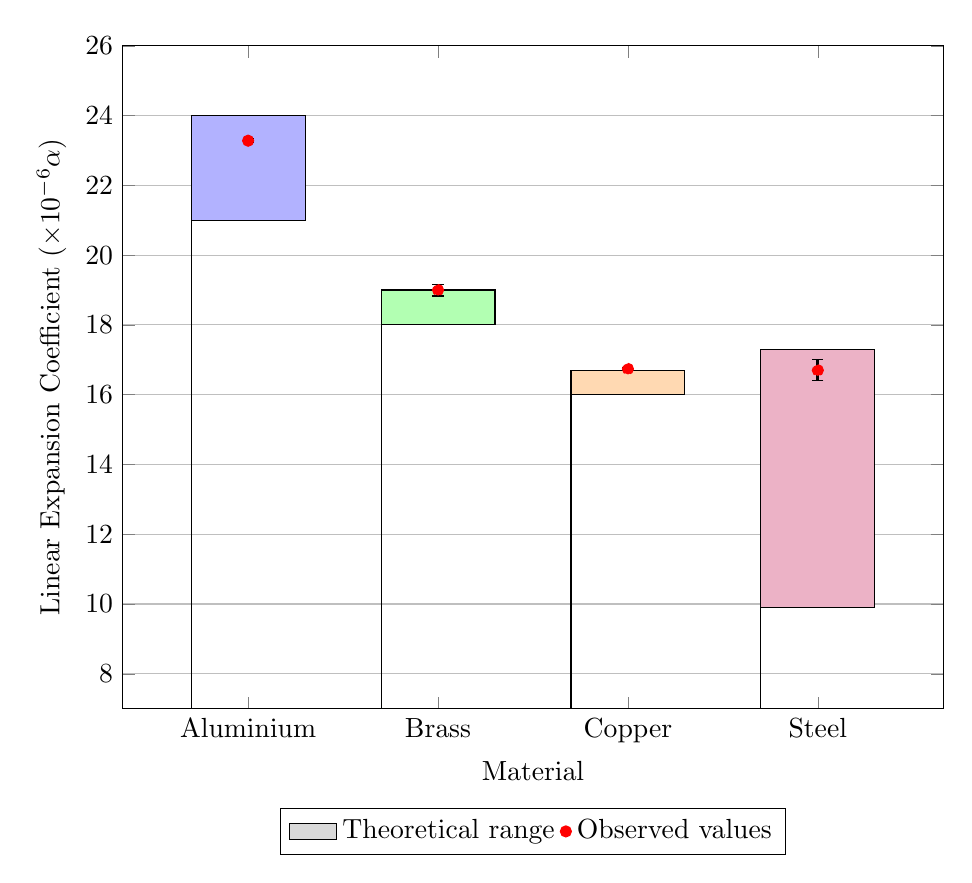
\begin{tikzpicture}
  % Set up the axis with custom dimensions, white background,
  % and y-axis starting at 7 for better visibility of error bars.
  \begin{axis}[
      width=12cm,
      height=10cm,              % Increased height for clear error bar visibility
      xlabel={Material},
      ylabel={Linear Expansion Coefficient ($\times 10^{-6} \alpha$)},
      xtick={1,2,3,4},
      xticklabels={Aluminium, Brass, Copper, Steel},
      ymin=7, ymax=26,          % y-axis range from 7 to 26
      ymajorgrids=true,
      axis background/.style={fill=white}, % Set the background to white instead of pink
      legend style={at={(0.5,-0.15)},anchor=north,legend columns=2},
  ]

  % Add legend entries:
  % - Theoretical range (displayed as a colored rectangle)
  % - Observed value with error bars (red dot with black error bars)
  \addlegendimage{area legend, fill=gray!30, draw=black}
  \addlegendentry{Theoretical range}
  \addlegendimage{only marks, mark=*, mark options={red}}
  \addlegendentry{Observed values}

  %-------------------------------
  % Plot theoretical ranges as colored rectangles
  % Each rectangle represents the range for the material.
  % The width of 0.6 units (from x-0.3 to x+0.3) centers the rectangle at the xtick.
  
  % Aluminium: theoretical range [21, 24]
  \addplot [draw=black, fill=blue!30] coordinates {
    (1-0.3,21) % Bottom left corner
    (1+0.3,21) % Bottom right corner
    (1+0.3,24) % Top right corner
    (1-0.3,24) % Top left corner
  } \closedcycle; % Close the cycle to form a rectangle

  % Brass: theoretical range [18, 19]
  \addplot [draw=black, fill=green!30] coordinates {
    (2-0.3,18)
    (2+0.3,18)
    (2+0.3,19)
    (2-0.3,19)
  } \closedcycle;

  % Copper: theoretical range [16, 16.7]
  \addplot [draw=black, fill=orange!30] coordinates {
    (3-0.3,16)
    (3+0.3,16)
    (3+0.3,16.7)
    (3-0.3,16.7)
  } \closedcycle;

  % Steel: theoretical range [9.9, 17.3]
  \addplot [draw=black, fill=purple!30] coordinates {
    (4-0.3,9.9)
    (4+0.3,9.9)
    (4+0.3,17.3)
    (4-0.3,17.3)
  } \closedcycle;

  %-------------------------------
  % Plot observed values with error bars:
  % The observed values are marked with red dots.
  % The error bars are drawn with a solid, dark black line and the caps are filled black.
  \addplot+[
      only marks,
      mark=*,
      mark options={red}, % Red dot for the observed value
      error bars/.cd,
      y dir=both,        % Error bars in both upward and downward directions
      y explicit,        % Use the explicit error value provided
      error bar style={color=black, line width=1pt, solid}, % Solid, dark black error bars
 %     error mark options={draw=black, fill=black, solid} % Filled black error bar caps
  ] coordinates {
      (1,23.28) +- (0,0.06) % Aluminium observed value with ±0.2 error
  };

  \addplot+[
      only marks,
      mark=*,
      mark options={red},
      error bars/.cd,
      y dir=both,
      y explicit,
      error bar style={color=black, line width=1pt, solid},
  ] coordinates {
      (2,19.0) +- (0,0.17) % Brass observed value with ±0.2 error
  };

  \addplot+[
      only marks,
      mark=*,
      mark options={red},
      error bars/.cd,
      y dir=both,
      y explicit,
      error bar style={color=black, line width=1pt, solid},
  ] coordinates {
      (3,16.74) +- (0,0.04) % Copper observed value with ±0.2 error
  };

  \addplot+[
      only marks,
      mark=*,
      mark options={red},
      error bars/.cd,
      y dir=both,
      y explicit,
      error bar style={color=black, line width=1pt, solid},
  ] coordinates {
      (4,16.7) +- (0,0.3) % Steel observed value with ±0.2 error
  };

  \end{axis}
\end{tikzpicture}












\noindent\rule{\linewidth}{0.4pt}

\newpage
\appendix
\section{Theoretical Values}
The expected values of $\alpha$ in \si{\per\celsius} are [4]:
\[
\begin{split}
\alpha_{\text{Steel}} &= (0.99 - 1.73) \times 10^{-5}\\
\alpha_{\text{Brass}} &= (1.8-1.9) \times 10^{-5}\\
\alpha_{\text{Aluminium}} &= (2.1 - 2.4) \times 10^{-5}\\
\alpha_{\text{Copper}} &= (1.6 - 1.67) \times 10^{-5}
\end{split}
\]

\section{Temperature of rod}\label{rodtemp}
The temperature of rod measured with the application of thermal paste is found to be ranging between $98~\si{\celsius}-99~\si{\celsius}$ (measured on 19 Mar 2025)






\end{document}
